
% confidence interval
% guassian with conficence region and with y axis 
\begin{center}
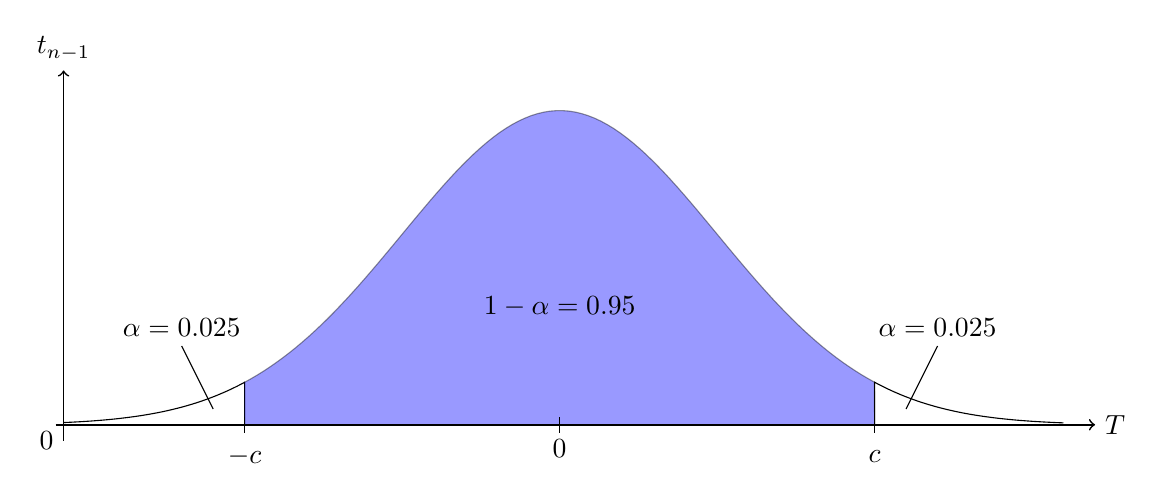
\begin{tikzpicture}[scale=2, y=5cm]
\draw[domain=-3.15:-2] (-3.15,0) plot[id=gauss1,samples=50]
(\x,{1/sqrt(2*pi)*exp(-0.5*(\x)^2)}) -- (-2,0);   
\draw[domain=-2:2,fill=blue,opacity=0.4] (-2,0) -- plot[id=gauss1, samples=100] (\x,{1/sqrt(2*pi)*exp(-0.5*(\x)^2)}) -- (2,0);   
\draw[domain=2:3.2] (2,0) --
plot[id=gauss3, samples=50] (\x,{1/sqrt(2*pi)*exp(-0.5*(\x)^2)});
\draw (2,-0.01) -- (2,0.01);    % ticks
\draw (-2,-0.01) -- (-2,0.01);
% ciritcal estimator values
\node at (2,-0.04) {$c$};
\node at (-2,-0.04) {$-c$};

% x-axis 1
\draw[->, semithick] (-3.2,0) -- (3.4,0) node[right] {$T$};  

% x-axis 2
%\draw[->, semithick] (-3.2,-0.1) -- (3.4,-0.1) node[right]
%{$T=\sqrt{n}\frac{\bar{x}-\bar{x}}{s}$}; 
% ticks on t
%\draw[-,semithick] (2,-0.11) -- (2,-0.09);
%\node at (2,-0.13)  {$c=2$};
%\draw[-,semithick] (-2,-0.11) -- (-2,-0.09);
%\node at (-2,-0.13)  {$-c=-2$};

%y-axis
\draw[->, semithick] (-3.15,-0.02) node[left] {$0$} -- (-3.15,0.45)
node[above] {$t_{n-1}$}; 

\draw[-,semithick] (0,-0.01) -- (0,0.01); % zero tick on x
% \draw[-,semithick] (0,-0.11) -- (0,0.-0.09); % zero tick on t
\node at (0,-0.03) {$0$};
% \node at (0,-0.13) {$0$};

% annotate alphas
\node at (0,0.15) {$1 - \alpha = 0.95$};
\draw (2.2,0.02) -- (2.4,0.1) node[above] {$\alpha = 0.025$};
\draw (-2.2,0.02) -- (-2.4,0.1) node[above] {$\alpha = 0.025$};
\end{tikzpicture} 
\end{center}
